\chapter{\label{ch:ch02}ПРАКТИЧЕСКАЯ ЧАСТЬ. ЭТАПЫ РАЗРАБОТКИ ИГРЫ.}

\section{\label{sec:ch02/sec01/sub01}Подготовка и установка окружения.}

Первый шаг на пути к созданию игры — установка \textbf{Unity Hub}~\cite{UnHub}. 

\textbf{Unity Hub} --- это центральное приложение для управления проектами, версиями Unity и лицензиями. 

После установки \textbf{Unity Hub}, можно было начать установку самой платформы \textbf{Unity}. Затем нужно было добавить наиболее стабильную версию \textbf{Unity} и выбрать при необходимости дополнительные компоненты, такие как поддержка различный ОС.

Для написания кода на C\# и работы с Unity была необходима интегрированная среда разработки, или же \textbf{IDE}. Было решено использовать \textbf{Visual Studio}~\cite{vscodeRu}, так как она отлично интегрируется с Unity и предоставляет все необходимые инструменты для разработки. Так как Visual Studio уже был установлен, нужно было дополнительно к нему загрузить рабочую нагрузку \textbf{Game development with Unity}~\cite{vsUn}. Это обеспечило установку всех нужных компонентов для работы с Unity и написания кода на C\#.

После установки всех необходимых инструментов был создан новый проект в Unity. В выборе шаблона проекта, выбор пал на 2D, т.к. необходимости в 3D пространстве не было и все можно было выполнить в 2D. 

Перед началом работы непосредственно с самим редактором Unity, необходимо было ознакомиться с интерфейсом и основными инструментами, необходимыми для разработки, т.к. изначально интерфейс мог казаться перегруженным различными панелями и кнопками. 

Основные инструменты разработки которые следовало изучить, были панели инструментов (см. рисунок~\ref{fig4}). : 
	\begin{itemize}
		\item Панель \textbf{Hierarchy} (1) показывает все объекты, находящиеся в текущей сцене.
		\item Панель \textbf{Scene} (2) позволяет визуально редактировать сцену. 
		\item Панель \textbf{Game} (3) используется для предпросмотра игры. 
		\item Панель \textbf{Inspector} (4) позволяет настраивать свойства выбранного объекта.
            \item Панель \textbf{Project} (5) помогает управлять файлами и папками проекта
            \item Панель \textbf{Console} (6) выводит ошибки, предупреждения и сообщения отладки.
	\end{itemize}

\begin{figure}[H]
	\centering
	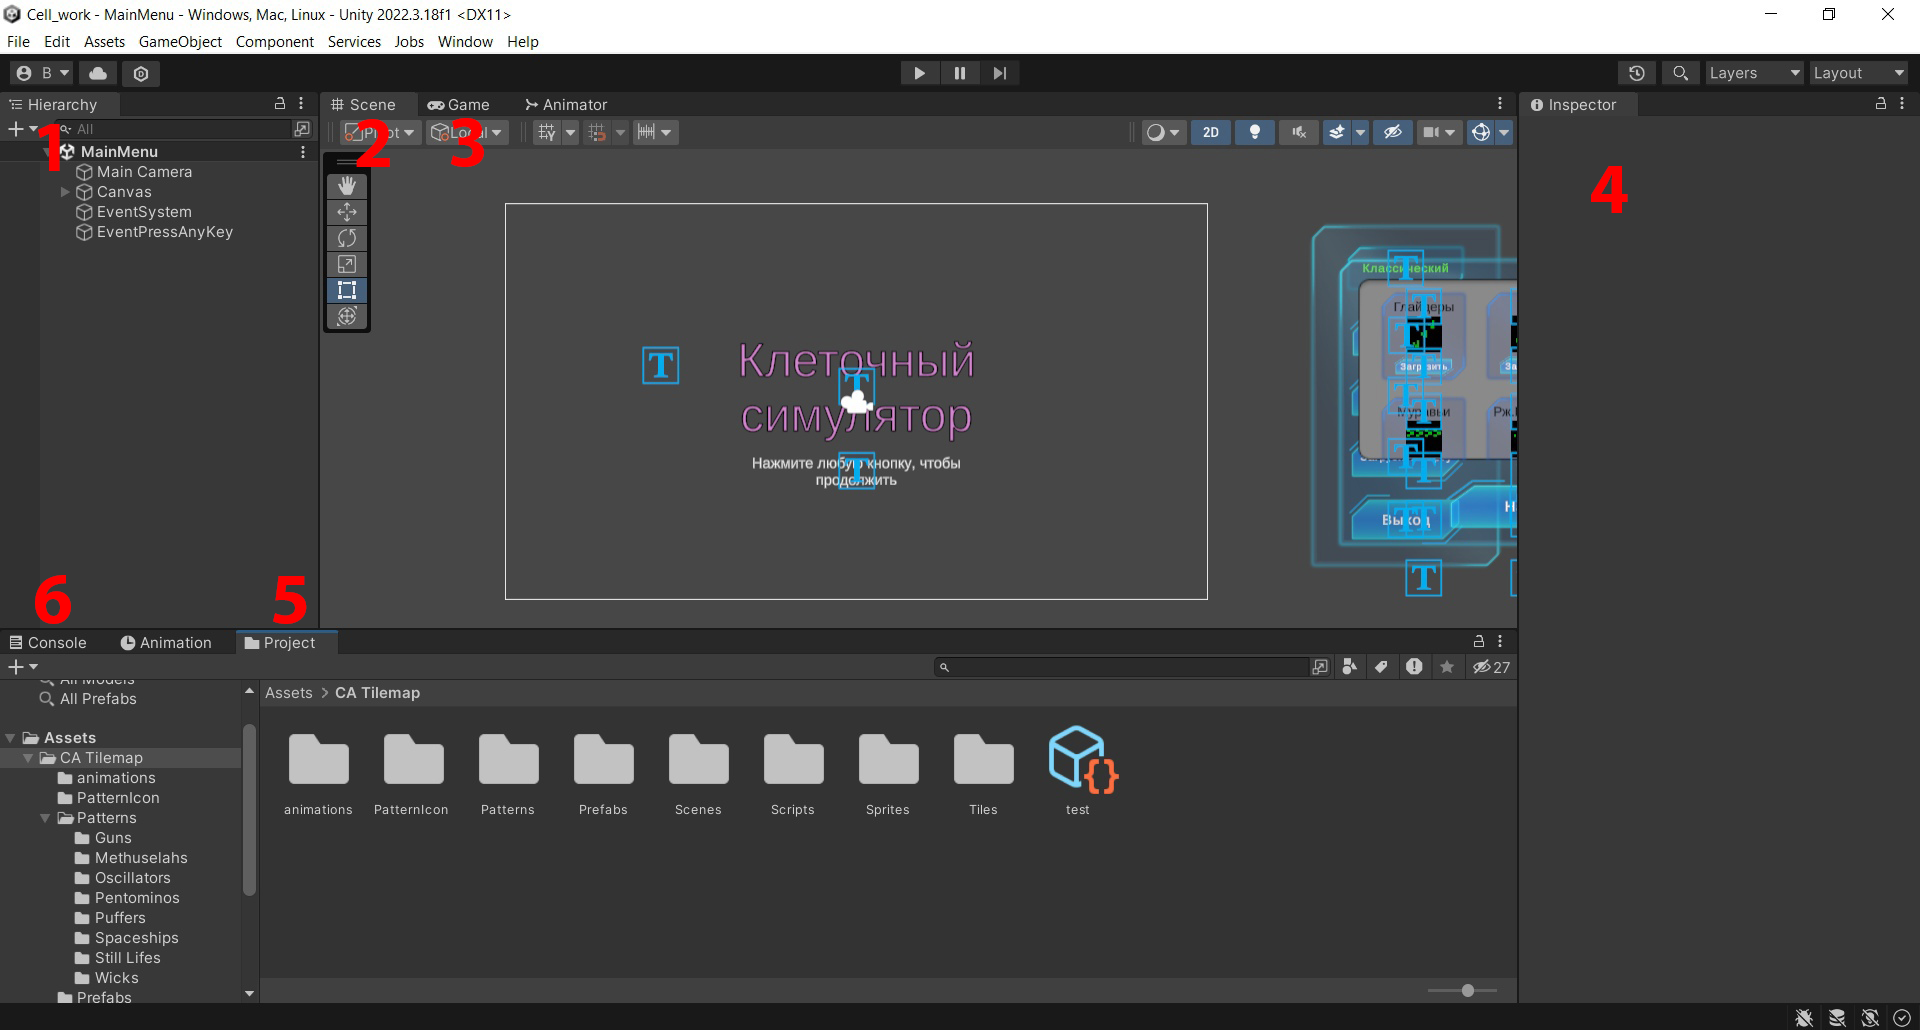
\includegraphics[width=1\textwidth]{images/Panels.png}  
	\caption{Панели инструментов.}
	\label{fig4}
\end{figure}

Далее появилась необходимость в изучении теории~\cite{OsnUnity}. В Unity есть несколько ключевых понятий, которые важно понимать с самого начала, т.к. большинство форумов и книг используют их. К ним относятся такие понятия как:
	\begin{itemize}
		\item \textbf{GameObject} --- это базовый объект в Unity, к которому можно прикреплять различные компоненты, такие как скрипты, физические свойства или визуальные элементы.
		\item \textbf{Component} --- это то, что добавляется к GameObject для придания ему различных свойств и функциональностей. 
		\item\textbf{Scene} --- это пространство, в котором располагаются все GameObjects. Игра может состоять из нескольких сцен, например, меню, уровня и экрана победы. 
		\item \textbf{Prefab} --- это шаблон объекта, который можно многократно использовать в проекте.
	\end{itemize}

После ознакомления с интерфейсом и основными понятиями, был сделан вывод, что рабочий стол организован и все необходимые инструменты настроены, что значительно упростило дальнейшую работу и позволило сосредоточиться на создании проекта.

\section{\label{sec:ch02/sec01/sub02}Реализация основного алгоритма клеточного автомата.}

После подготовки и установки окружения была выполнена реализация базового алгоритма клеточного автомата. Этот алгоритм представляет собой математическую модель, которая имитирует поведение клеток на двумерной решетке. Каждая клетка может быть либо <<живой>>, либо <<мертвой>>, и её состояние в следующем поколении зависит от состояния соседних клеток.

Вначале было проведено теоретическое изучение основных правил <<Игры жизни>>~\cite{GameLife}. Эти правила включали в себя: смерть клетки от одиночества при наличии менее двух живых соседей, выживание при двух или трёх живых соседях, смерть от перенаселения при наличии более трёх живых соседей и возрождение мёртвой клетки при наличии ровно трёх живых соседей.

После этого началась разработка алгоритма. В Unity был создан скрипт на языке C\#, который реализовывал логику обновления состояния клеток. Вместо использования классического двумерного массива, был использован массив, хранящий координаты клеток из \textbf{Tilemap}~\cite{tilemap}. Это позволило учитывать специфические особенности Unity и обеспечить более точное взаимодействие с визуальной частью игры. В ходе разработки использовался скрипт \textbf{GameBoard.cs}(см. \textbf{\textsc{ПРИЛОЖЕНИЕ}} на стр.~\pageref{code:brgame}), в котором хранилась логика основной симуляции. В этом скрипте были В функции \textbf{UpdateState()}(см. \textbf{\textsc{ПРИЛОЖЕНИЕ}} на стр.~\pageref{code:brgame} строки 118-164) в котором происходило обновление их состояния и визуализации текущего состояния на \textbf{Tilemap}, а функция \textbf{SetPattern()}(см. \textbf{\textsc{ПРИЛОЖЕНИЕ}} на стр.~\pageref{code:brgame} строки 66-82) отвечала за начальную настройку массива клеток случайными значениями.  В частности, использовались методы для определения состояния клетки и её соседей, такие как \textbf{IsAlive()} и \textbf{CountNeighbors()}(см. \textbf{\textsc{ПРИЛОЖЕНИЕ}} на стр.~\pageref{code:brgame} строки 210-213 и строки 166-198).

\textbf{Tilemap} в Unity оказался удобным инструментом для визуализации клеточного автомата. Это компонент, который позволяет легко создавать и редактировать двумерные сетки, используя тайлы (маленькие графические элементы). Для визуализации состояния клеток был создан новый \textbf{Tilemap} в сцене Unity. Этот компонент позволил упрощённое отображение и управление клетками на игровом поле.



Был написан скрипт \textbf{TilemapClickHandler.cs}(см. \textbf{\textsc{ПРИЛОЖЕНИЕ}} на стр.~\pageref{code:click}), который обеспечивал взаимодействие с клетками на уровне визуализации. Этот скрипт позволял пользователю кликать по клеткам, тем самым создавая их, что делало игровой опыт более интерактивным и удобным и в то же время демонстрировала работу алгоритма.

Во время тестирования и отладки были выявлены несколько проблем. Например, неправильное определение количества соседей у граничных клеток и ошибки при копировании массивов, что приводило к некорректному обновлению состояния клеток. Эти проблемы были исправлены в ходе тщательной отладки кода. Были также внедрены различные методы для проверки корректности работы алгоритма и его соответствия правилам <<Игры жизни>>.

Для обеспечения плавной работы алгоритма на разных устройствах была проведена оптимизация кода. Основное внимание уделялось минимизации количества операций в основном цикле обновления, использованию эффективных методов для копирования и обновления массивов, а также оптимизации рендеринга клеток. В результате проведённых оптимизаций алгоритм стал работать более плавно и эффективно, даже при увеличении размера поля и частоты обновления.

Таким образом алгоритм клеточного автомата <<Игры жизни>> был реализован, протестирован и визуализирован с использованием Tilemap, что позволило перейти к следующим этапам разработки проекта.

\section{\label{sec:ch02/sec01/sub03}Создание пользовательского интерфейса (UI)}

После реализации и проверки основной механики игры, началось выполнение этапа разработки пользовательского интерфейса (UI) для игры <<Игра жизни>>. 
Этот этап включал в себя создание интерактивных элементов, которые позволяли пользователям управлять симуляцией, редактировать, загружать и генерировать их, а также изменять параметры клеточного автомата. Основной задачей было сделать интерфейс интуитивно понятным и удобным для пользователя.

Для обеспечения удобства использования и отзывчивости интерфейса были изучены и применены практики UI/UX-дизайна~\cite{UI/Ux}, чтобы интерфейс был интуитивно понятным и легко читаемым. Особое внимание было уделено размеру и расположению кнопок, а также цветовой гамме интерфейса.

Для начала было решено создать основные элементы управления симуляцией. В Unity на главном экране игры было разработано основное меню, которое включало несколько ключевых кнопок:
        \begin{itemize}
		\item \textbf{Редактор} --- переход в режим редактирования клеточного автомата..
		\item \textbf{Случайная генерация} --- создание случайного начального состояния. 
		\item\textbf{Загрузить карту} --- загрузка предварительно сохраненных паттернов. 
		\item \textbf{Выход} --- завершение работы программы.
            \item \textbf{Помощь} --- загрузка описания проекта и автора.
	\end{itemize}

Эти элементы управления были реализованы с использованием стандартных UI-компонентов Unity, таких как Button и Panel.

Первым делом для удобства пользователей была создана отдельная панель, где можно было выбрать предопределенные паттерны клеток. На этой панели отображались кнопки с изображениями и названиями паттернов, таких как Глайдеры, Иви, Блинкер, Муравьи, Ружье Госпера и Вакуумная пушка~\cite{pattern}. Пользователь мог загрузить выбранный паттерн, нажав соответствующую кнопку <<Загрузить>>. Эта функциональность была реализована с помощью скрипта \textbf{LevelTransition.cs} (см. \textbf{\textsc{ПРИЛОЖЕНИЕ}} на стр.~\pageref{code:lvl})

Следом была создана отдельная панель, где пользователь мог задать размер карты и случайным образом сгенерировать начальное состояние клеток. На этой панели размещались кнопки для выбора размеров карты (20x20, 50x50, 100x100) и кнопка <<Сгенерировать>>, которая инициализировала случайное распределение живых клеток на карте. Эта функциональность была реализована с помощью скрипта \textbf{RandomButton.cs}. (см. \textbf{\textsc{ПРИЛОЖЕНИЕ}} на стр.~\pageref{code:rndB}). 

Для режима редактирования была создана отдельная сцена где пользователь мог задать размер карты перед началом редактирования и так же для интерактивного управления клетками была реализована возможность изменения состояния клеток с помощью кликов мыши. Эта функциональность была реализована с помощью скриптов \textbf{TilemapClickHandler.cs} и \textbf{EditorStartMap.cs}. (см. \textbf{\textsc{ПРИЛОЖЕНИЕ}} на стр.~\pageref{code:strMap})

После разработки основных элементов интерфейса было проведено тщательное тестирование. Были выявлены и исправлены ошибки, связанные с отображением информации и взаимодействием с элементами управления. Тестирование проводилось на различных устройствах, чтобы убедиться в корректной работе интерфейса на всех поддерживаемых разрешениях.


\section{\label{sec:ch02/sec01/sub04}Блок-схема.}

Блок-схема <<Игры жизни>> Джона Конвея иллюстрирует процесс обновления состояния клеток на игровом поле. Алгоритм основан на простых правилах, которые определяют, будет ли клетка <<живой>> или <<мертвой>> в следующем поколении, в зависимости от состояния её соседей. Данная блок-схема показывает основные этапы работы алгоритма, начиная с инициализации и заканчивая обновлением состояния клеток (см. рисунок~\ref{fig4}). 

\begin{figure}[H]
	\centering
	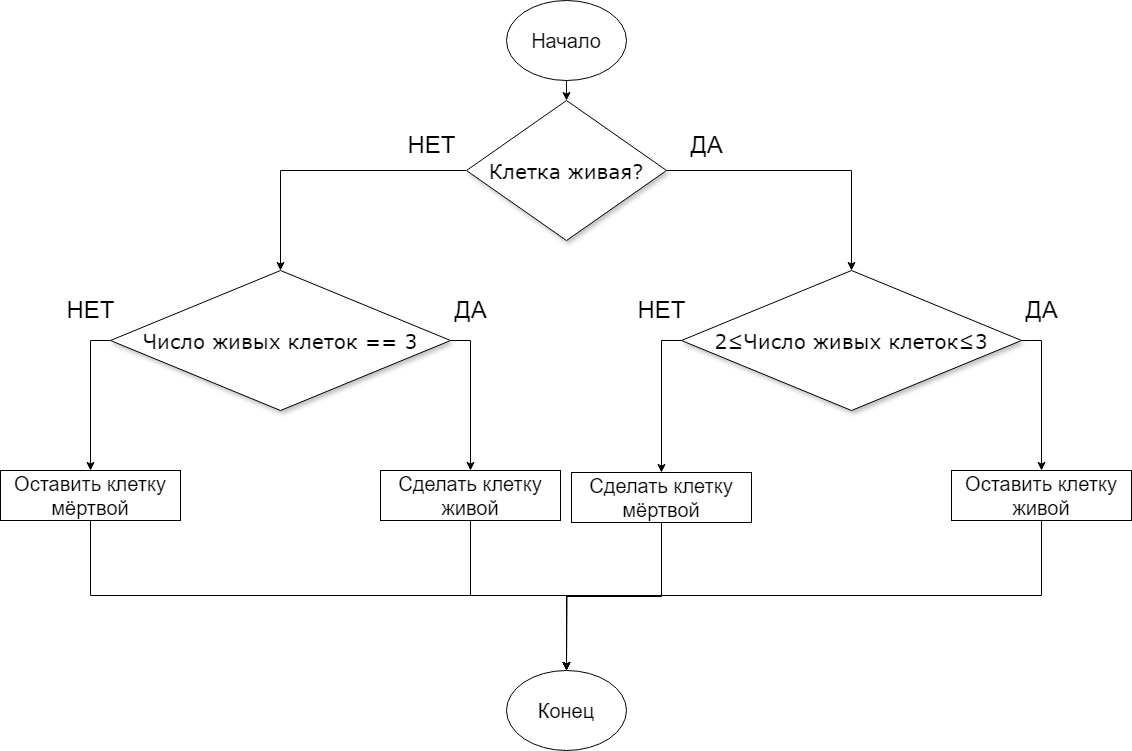
\includegraphics[width=1\textwidth]{images/БлокСхема.png}  
	\caption{Блок схема алгоритма <<Игры жизни>>.}
	\label{fig4}
\end{figure}

\section{\label{sec:ch02/sec01/sub05}Сборка программы}

Сборка программы является предфинальным этапом разработки проекта в Unity. На этом этапе проект подготавливается к запуску на различных платформах, таких как Windows, macOS, Linux, iOS и других. В данном разделе описаны шаги по сборке программы, начиная с настройки проекта и заканчивая созданием исполняемых файлов.

Перед сборкой программы необходимо было убедиться, что все параметры проекта настроены правильно. Для этого в Unity используется меню <<File > Build Settings...>>. В открывшемся окне можно выбрать платформу, на которую будет производиться сборка, а также настроить основные параметры.

\begin{figure}[H]
	\centering
	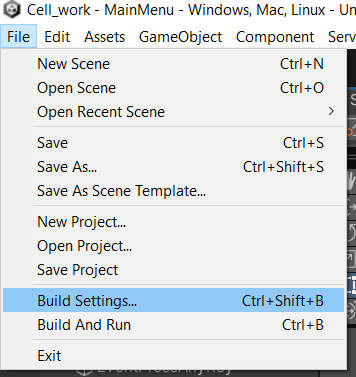
\includegraphics[width=0.3\textwidth]{images/build1.png}  
	\caption{Открытие меню Build Settings.}
	\label{fig5}
\end{figure}

В окне <<Build Settings>> выберется платформа, на которую будет производиться сборка (например, PC, Mac \& Linux Standalone для Windows и macOS, или Android для мобильных устройств). Были добавлены все необходимые сцены в раздел <<Scenes In Build>>, нажав на кнопку <<Add Open Scenes>>. Необходимо было убедитесь, что все сцены, которые должны быть включены в сборку, добавлены в этот список.

\begin{figure}[H]
	\centering
	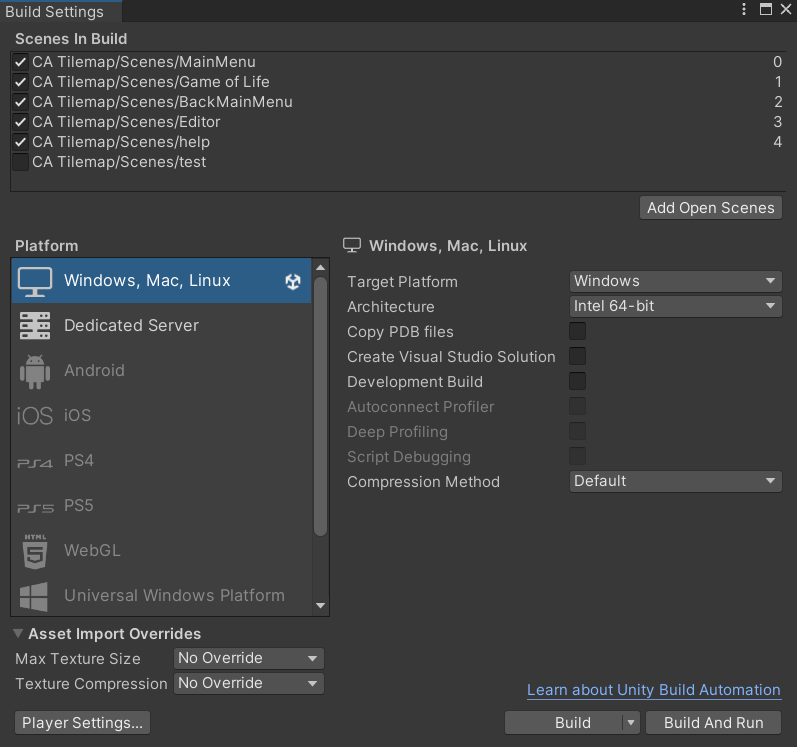
\includegraphics[width=0.4\textwidth]{images/build2.png}  
	\caption{Окно Build Settings.}
	\label{fig5}
\end{figure}

В зависимости от выбранной платформы могут потребоваться дополнительные настройки. Для Windows и macOS также можно было настроить параметры отображения, значки и другие параметры.

После настройки всех параметров нажав на кнопку <<Build>>, Unity предложило выбрать папку, в которую будет сохранен скомпилированный проект.Выбрав подходящее место, начался процесс сборки.

Скомпилированным проект в папке будет иметь такой вид (см. рисунок~\ref{fig6}). 
\begin{figure}[H]
	\centering
	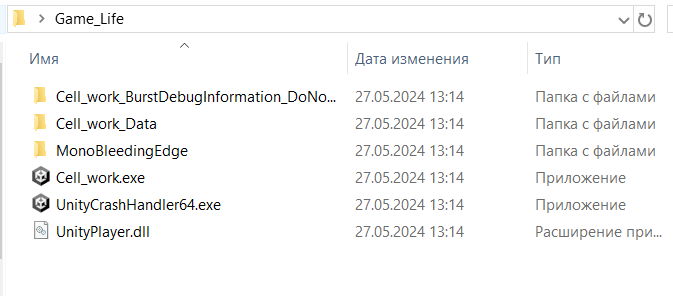
\includegraphics[width=0.6\textwidth]{images/dir.png}  
	\caption{Директория с исполняемым файлом.}
	\label{fig6}
\end{figure}

\section{\label{sec:ch02/sec01/sub06}Тестирование программы}

После завершения сборки в конце необходимо было протестировать скомпилированный проект на целевой платформе. Запустить созданный исполняемые файлы на соответствующей операционной системе и следовало убедиться, что программа работает корректно. Проверив все основные функции и элементы интерфейса, убедиться в отсутствии ошибок. 

При запуске игры нас встречает главное меню (см. \textbf{\textsc{ПРИЛОЖЕНИЕ}} на стр.~\pageref{MainM}).

При нажатии на кнопку <<Редактор>> меняется экран. На нём отображена возможность редактирования игрового поля и задания размеров карты (см. \textbf{\textsc{ПРИЛОЖЕНИЕ}} на стр.~\pageref{Editor}). 

При нажатии на кнопку <<Случайная Генерация>> появляется панель. На ней отображены настройки размера карты (см. \textbf{\textsc{ПРИЛОЖЕНИЕ}} на стр.~\pageref{rand}). 

При нажатии на кнопку <<Загрузить карту>> появляется панель. На ней отображены кнопки выбора предопределенных паттернов и загрузки карты (см. \textbf{\textsc{ПРИЛОЖЕНИЕ}} на стр.~\pageref{downl}). 

Основное игровое поле выглядит следующим образом (см. \textbf{\textsc{ПРИЛОЖЕНИЕ}} на стр.~\pageref{map}).

Пример ситуации, когда запускается симуляция <<Игры жизни>>, некоторые клетки появляются, исчезают или остаются неизменными в зависимости от правил, приведены ниже (см. \textbf{\textsc{ПРИЛОЖЕНИЕ}} на стр.~\pageref{uim}).
